\chapter{二次哈密顿量的精确相空间流}
\label{ch:quadratic}

\begin{learningobjectives}
完成本章后，读者应能：
\begin{enumerate}
  \item 证明二次哈密顿量的 Wigner 演化严格等于经典 Liouville 演化；
  \item 用辛矩阵传播相空间均值和协方差；
  \item 区分“高斯态保持高斯”和“任意 Wigner 函数按线性流精确搬运”；
  \item 用守恒量、均值和协方差检验数值传播程序。
\end{enumerate}
\end{learningobjectives}

\section{一般二次哈密顿量}

二次玻色哈密顿量与连续变量高斯态的辛演化属于同一线性正则结构；
较完整的连续变量量子信息表述可参见\cite{Weedbrook2012}。

沿用第2章的无量纲模式正交分量，把 $M$ 模写成 $2M$ 维列向量
\begin{equation}
  \hat{\bm R}=(\hat Q_1,\hat P_1,\ldots,\hat Q_M,\hat P_M)^T,
\end{equation}
满足
\begin{equation}
  \comm{\hat R_j}{\hat R_k}=\ii\Omega_{jk}.
\end{equation}
一般的时变二次哈密顿量可写成频率单位的形式
\begin{equation}
  \Hhat(t)=\hbar\left[
  \frac12\hat{\bm R}^{\mathsf T}G(t)\hat{\bm R}
  +\bm h(t)^{\mathsf T}\hat{\bm R}+c(t)\right],
  \label{eq:quadratic-hamiltonian}
\end{equation}
其中 $G=G^{\mathsf T}$，$G$ 与 $\bm h$ 的量纲是频率。由于 Weyl 对称化，频率函数 $\mathcal H_W\equiv H_W/\hbar$ 就是把 $\hat{\bm R}$ 替换为 $\bm R$ 后的括号内二次函数。若改用有量纲的坐标--动量，则应把相应尺度和 $1/\hbar$ 一并恢复，不能与本段的 $G$ 直接混用。

Moyal 展开中的 $\Lambda^3$ 及更高项至少需要哈密顿量的三阶导数，因此全部为零。精确 Wigner 方程退化为
\begin{equation}
  \pder{W}{t}=\{\mathcal H_W,W\}_{\mathrm{PB}}.
  \label{eq:quadratic-liouville}
\end{equation}
它的特征线满足经典 Hamilton 方程
\begin{equation}
  \dot{\bm R}=\Omega\bigl[G(t)\bm R+\bm h(t)\bigr].
  \label{eq:linear-hamilton-equation}
\end{equation}
这里没有作 TWA 截断；经典形式来自 Moyal 级数精确终止。

\begin{intuitionbox}
二次哈密顿量不能在相空间中产生新的细尺度折叠。它只对已有分布作旋转、剪切、压缩和平移。因此，即使初态是带负值的 Fock 态 Wigner 函数，其精确演化仍可由同一线性辛流搬运。
\end{intuitionbox}

\section{辛传播矩阵}

齐次部分的基解矩阵 $S(t,t_0)$ 满足
\begin{equation}
  \pder{S(t,t_0)}{t}=\Omega G(t)S(t,t_0),
  \qquad S(t_0,t_0)=I.
\end{equation}
解可写成
\begin{equation}
  \bm R(t)=S(t,t_0)\bm R(t_0)+\bm r_c(t),
  \label{eq:affine-symplectic-flow}
\end{equation}
其中 $\bm r_c$ 由驱动 $\bm h$ 决定。传播保持对易关系，因而
\begin{equation}
  S\Omega S^{\mathsf T}=\Omega.
  \label{eq:symplectic-condition}
\end{equation}
满足\cref{eq:symplectic-condition} 的矩阵称为辛矩阵。

对均值 $\bm d$ 和协方差 $V$，传播规则为
\begin{align}
  \bm d(t)&=S\bm d(t_0)+\bm r_c(t),\\
  V(t)&=SV(t_0)S^{\mathsf T}.
  \label{eq:gaussian-moment-propagation}
\end{align}
若初态为高斯态，\cref{eq:gaussian-moment-propagation} 已经给出全部状态信息；若初态非高斯，均值和协方差仍按该式演化，但不能由它们重建完整状态。

\section{谐振子的相空间旋转}

\begin{equation}
  \Hhat=\hbar\omega\left(\had\ha+\frac12\right)
  =\frac{\hbar\omega}{2}(\hat Q^2+\hat P^2).
\end{equation}
Hamilton 方程为 $\dot Q=\omega P$、$\dot P=-\omega Q$，所以
\begin{equation}
  \begin{pmatrix}Q(t)\\P(t)\end{pmatrix}
  =
  \begin{pmatrix}
    \cos\omega t&\sin\omega t\\
    -\sin\omega t&\cos\omega t
  \end{pmatrix}
  \begin{pmatrix}Q(0)\\P(0)\end{pmatrix}.
  \label{eq:harmonic-symplectic-rotation}
\end{equation}
复振幅因此满足 $\alpha(t)=\alpha(0)\ee^{-\ii\omega t}$。相干态 Wigner 云团作刚性旋转，真空宽度不变，粒子数估计量 $|\alpha|^2-1/2$ 沿每条轨迹都守恒。

\begin{figure}[htbp]
  \centering
  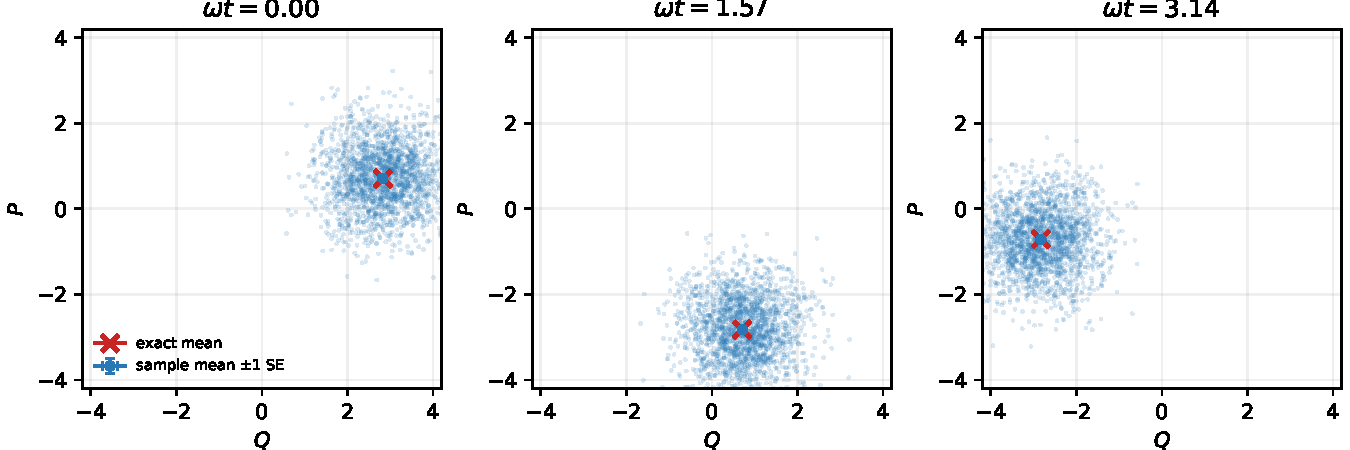
\includegraphics[width=0.94\textwidth]{figures/ch05/harmonic_wigner_rotation.pdf}
  \caption[谐振子二次流的 Wigner 样本基准]{相干态 Wigner 样本在谐振子二次哈密顿量下的精确旋转，参数为 $\alpha_0=2+0.5\ii$、$\omega=1$。蓝点为 $2000$ 条可视化轨迹的截面，圆点及误差棒为全部 $20000$ 条轨迹给出的样本均值及其 $\pm1$ 标准误，红叉为解析均值。该基准只检验可精确抽样的高斯初态与二次传播；图由 \texttt{code/ch05\_quadratic/harmonic\_wigner.py} 实际计算。}
  \label{fig:harmonic-wigner-rotation}
\end{figure}

\section{实际数值验证}

\cref{fig:harmonic-wigner-rotation} 使用 $\alpha_0=2+0.5\ii$、$\omega=1$ 和固定随机种子。样本通过
\begin{equation}
  \alpha^{(s)}(0)=\alpha_0+\frac{\xi_1^{(s)}+\ii\xi_2^{(s)}}{2}
\end{equation}
生成，再用解析旋转传播。程序输出的验证结果为
\begin{align}
  \max_t|\overline\alpha(t)-\alpha_0\ee^{-\ii t}|
  &=5.51\times10^{-3},\\
  \widehat{\qavg{\hat n}}&=4.25275,
  \qquad \qavg{\hat n}_{\mathrm{exact}}=4.25.
\end{align}
三个抽查时刻的 $Q,P$ 样本方差位于 $0.4985$ 至 $0.5051$，与真空方差 $1/2$ 相容。数据保存在 \texttt{data/ch05/harmonic\_wigner\_metrics.json}。

这些偏差来自有限样本，不是动力学截断。若把轨迹数扩大四倍，均值误差的典型尺度应约缩小一半。由于传播使用解析解，时间离散误差在本实验中为零。

\begin{numericalbox}
二次模型是测试 TWA 软件的首选：初态抽样、漂移、观测量排序和解析答案可以同时检查。若代码不能在此处保持协方差和二次守恒量，就不应直接用于非线性多体模型。
\end{numericalbox}

\section{自由膨胀、剪切与压缩}

这里临时回到有量纲的位置--动量对：自由粒子哈密顿量 $H=p_x^2/(2m)$ 给出
\begin{equation}
  x(t)=x(0)+\frac{t}{m}p_x(0),
  \qquad p_x(t)=p_x(0),
\end{equation}
对应相空间剪切。倒置谐振子产生双曲伸缩，一个方向指数放大，另一个方向指数压缩；演化仍然精确，但数值误差也会沿不稳定方向放大。含 $a^2+a^{\dagger2}$ 的参量放大哈密顿量同样是二次的，它可以产生压缩和纠缠，却无需高阶 Moyal 项。

这说明“精确经典相空间流”并不等价于“没有量子效应”。量子性可以完全存在于初态协方差、负 Wigner 结构和观测量排序中；二次哈密顿量只是不会生成超出线性辛变换的新非高斯结构。

\section{数值积分的辛性}

对时变或大规模二次系统，通常需要数值求解\cref{eq:linear-hamilton-equation}。除了减小时间步长，还应检查
\begin{equation}
  \epsilon_{\mathrm{sp}}
  =\lVert S\Omega S^{\mathsf T}-\Omega\rVert,
  \label{eq:symplectic-error}
\end{equation}
以及适用时的能量误差。普通高阶积分器可以在短时间内具有很小局域误差，却缓慢破坏辛结构；辛积分器更适合超长时间的哈密顿量传播。对含指数不稳定方向的系统，还应区分真实的物理放大与浮点误差放大。

\begin{warningbox}
二次哈密顿量下“Wigner 演化精确”不意味着有限轨迹 Monte Carlo 没有误差，也不意味着高斯协方差足以描述非高斯初态。精确性只针对连续 Wigner 方程与经典 Liouville 方程的一致。
\end{warningbox}

\section*{本章小结}

二次哈密顿量的 Moyal 级数精确终止，Wigner 函数沿线性仿射辛流传播。高斯态可以只传播均值和协方差，任意非高斯态则需传播完整分布或样本。谐振子数值实验验证了真空宽度、相空间旋转和正规排序粒子数，为后续非线性基准建立了零截断误差的参照。

\begin{exercises}
  \item 验证谐振子旋转矩阵满足\cref{eq:symplectic-condition}。
  \item 推导自由粒子的协方差 $V(t)$，说明位置方差为何出现 $t^2$ 项。
  \item 对倒置谐振子求 $S(t)$，找出稳定和不稳定方向。
  \item 证明辛传播保持高斯态不确定关系\cref{eq:uncertainty-matrix}。
  \item 修改配套程序，把解析旋转替换为 Euler 法，测量能量误差和辛误差怎样随时间步长变化。
\end{exercises}
